\documentclass[sigconf]{acmart}

\usepackage{booktabs} % For formal tables

\usepackage{amsmath, amssymb, amsthm, enumitem, breqn, bm, geometry, subcaption}


% Copyright
%\setcopyright{none}
%\setcopyright{acmcopyright}
%\setcopyright{acmlicensed}
\setcopyright{rightsretained}
%\setcopyright{usgov}
%\setcopyright{usgovmixed}
%\setcopyright{cagov}
%\setcopyright{cagovmixed}


% DOI
\acmDOI{10.1145/nnnnnnn.nnnnnnn}

% ISBN
\acmISBN{978-x-xxxx-xxxx-x/YY/MM}


%Conference
\acmConference[GECCO '18]{the Genetic and Evolutionary Computation
Conference 2018}{July 15--19, 2018}{Kyoto, Japan}
\acmYear{2018}
\copyrightyear{2018}


\acmArticle{4}
\acmPrice{15.00}

% These commands are optional
%\acmBooktitle{Transactions of the ACM Woodstock conference}
\editor{Jennifer B. Sartor}
\editor{Theo D'Hondt}
\editor{Wolfgang De Meuter}


\begin{document}
\title{Learning an Evolvable Genotype-Phenotype Mapping}

\author{Matthew Andres Moreno}
\orcid{0000-0003-4726-4479}
\affiliation{%
  \institution{BEACON Center}
  \streetaddress{Michigan State University}
}
\email{mmore500@msu.edu}

\author{Wolfgang Banzhaf}
\orcid{0000-0002-6382-3245}
\affiliation{%
  \institution{BEACON Center}
  \streetaddress{Michigan State University}
}
\email{banzhafw@msu.edu}

\author{Charles Ofria}
\orcid{0000-0003-2924-1732}
\affiliation{%
  \institution{BEACON Center}
  \streetaddress{Michigan State University}
}
\email{ofria@msu.edu}

\begin{abstract}
Two schemes for automatic generation of evolvable genotype-phenotype mappings are presented. Both schemes use an artificial neural network (ANN) autoencoder trained on phenotypes harvested from fitness peaks as the basis for a genotype-phenotype mapping. In the first, the decoder segment of a bottlenecked autoencoder is used as the genotype-phenotype mapping. In the second, a denoising autoencoder is used as the genotype-phenotype mapping. Automatic generation of evolvable genotype-phenotype mappings are demonstrated on the $n$-legged table problem, a toy problem that defines a simple rugged fitness landscape, and the Scrabble string problem, a more complicated problem that serves as a rough model for linear genetic programming. For both problems, the automatically generated genotype-phenotype mappings are found to enhance evolvability.

\end{abstract}

%
% The code below should be generated by the tool at
% http://dl.acm.org/ccs.cfm
% Please copy and paste the code instead of the example below.
%
\begin{CCSXML}
<ccs2012>
<concept>
<concept_id>10010147.10010257.10010293.10011809.10011815</concept_id>
<concept_desc>Computing methodologies~Generative and developmental approaches</concept_desc>
<concept_significance>500</concept_significance>
</concept>
<concept>
<concept_id>10010147.10010257.10010293.10011809.10011812</concept_id>
<concept_desc>Computing methodologies~Genetic algorithms</concept_desc>
<concept_significance>300</concept_significance>
</concept>
</ccs2012>
\end{CCSXML}

\ccsdesc[500]{Computing methodologies~Generative and developmental approaches}
\ccsdesc[300]{Computing methodologies~Genetic algorithms}

\keywords{genetic algorithms, adaptive representations, indirect encodings, genotype-phenotype map, evolvability, deep learning}

\maketitle

\section{Introduction} \label{sec:background}

Successful evolutionary search depends the production of heritable, novel phenotypic variation, some of which must not be severely deleterious.
Without any heritable variation --- or even just without any viable heritable variation --- evolution stagnates.
The capacity of a population to generate viable heritable phenotypic variation is referred to as evolvability.

Different evolving systems can exhibit different degrees of evolvability.
Different digital evolution systems exhibit different evolvability TODO
Natural systems, in particular, are thought to generally exhibit greater evolvability than digital evolution systems \cite{mengistu2016evolvability}.
Let us examine a pair of biological examples of non-arbitrary phenotypic outcomes under mutation to build our intuition for evolvability.

A developmental constraint against certain non-viable phenotypic variation in  \textit{Drosophilia melangoster} was discovered through artificial selection experiments \cite{coyne1987lack, tuinstra1990lack}.
In these experiments,  researchers were able to successfully select for bilaterally symmetric phenotypic criteria, such as overall smaller eyes, but were unable to successfully select for bilaterally asymmetric phenotypic traits, such as different-sized eyes.
Tuinstra et al. hypothesize that the very nature of the developmental process constrains the phenotypic variation that can be observed in offspring, in this case curtailing the abundance of offspring that lack bilateral symmetry.
Specifically, they hypothesize that a lack of bilateral symmetry-breaking information during the embryological development of *Drosophila* explains the negative result of artificial selection for bilaterally asymmetric phenotypic traits.
In this way, the distribution of phenotypic diversity in offspring is biased away from (likely non-viable) asymmetric variation.

In addition to qualities that constrain against non-viable mutational outcomes, biological organisms can possess qualities that facilitate significant heritable variation for a phenotypic trait.
Somatotropin, also known as growth hormone, is well known for its widespread anabolic effects on tissues throughout the body.
Mutations affecting the regulatory pathways that regulate somatotropin production and release, the receptors and cell signaling components that mediate cellular response to somatotropin, and the protein itself all provide avenues for significant heritable variation in body size \cite{devesa2016multiple}.
Dog breeds exhibit a range of body weights spanning nearly an entire order of magnitude.
Indeed, among certain groups of dogs, much of this variation can be explained by just six genes, several of which are associated with pathways somatotropin participates in \cite{rimbault2013derived}.
The presence of hormonal signaling pathways like those somatotropin participates in can be viewed as making a broad range of heritable phenotypic variation more readily realizable via mutation.

A general consensus exists in the literature that evolvability stems from traits that facilitate the generation of \textit{novel} heritable phenotypic variation that is \textit{viable} \cite{tarapore2015evolvability}.

[describe evolvability signature]
Tarapore et al. introduced an evolvability measure that attempts to take a more clear-eyed view of both of the primary aspects of evolvability: the amount of heritable variation among offspring and the fitness effects of that variation \cite{tarapore2015evolvability}.
They forgo use of a scalar metric to describe evolvability, instead reporting evolvability using what they term a ``signature.''
Essentially, the signature is a two-dimensional heatmap presenting the changes in phenotypic form and fitness observed in individual offspring from a single parent.
Normalized mutual information between the phenotypic states of parent and offspring is used to quantify the amount of change in phenotypic form observed in an offspring.
Proportion decrease in fitness is used to quantify the fitness difference between parent and offspring.
For a highly evolvable individual, we would expect to see offspring occurring with significant frequency in the corner of the heatmap indicating significant change in phenotypic form with slight or no loss of fitness.
The evolvability signature provides a nuanced snapshot of evolvability, allowing for interaction between the two primary components of evolvability to be visualized.
Such information can be highly diagnostic, for example alerting researchers to phenomena that might appear falsely promising using other metrics, such as genetic changes that alter phenotypic form significantly but at great cost to fitness or genetic changes that are beneficial to fitness but fail to uncover novel phenotypic form.
[ADD EXAMPLE READING IT FIGURE]

To rival that of natural systems
Evolvability is desirable in artificial evolution systems for practical ends --- developing more evolvable artificial evolution systems will allow evolutionary algorithms to tackle more sophisticated problems more effectively.
Understanding evolvability is also important to scientific ends for evolutionary biologists and evolutionary computing researchers alike  \cite{mengistu2016evolvability, pigliucci2008evolvability}.

\subsection{Genotype-Phenotype Map and Evolvability}

In biological science, a distinction is drawn between an organism's genotype and phenotype.
Phenotype refers to an organism's observable characteristics (morphological, behavioral, physiological, chemical, etc.) that govern its interaction with the environment and ultimately determine its fitness.
Genotype refers the heritable information that influences the phenotype displayed by the individual, i.e. the organism's DNA.
Development is the process through which an organism's genotype shapes (but does not completely determine due to environmental influence) its phenotype.
It is useful to abstract development as a mathematical function that takes genetic information as its input and outputs phenotypic characteristics.
This mathematical function representing development is referred to as the genotype-phenotype map \cite{alberch1991genes}.

The nature of the genotype-phenotype map employed in an evolving system is thought to influence that system's evolvability \cite{pigliucci2010genotype}.
Let us discuss three theoretical constructs that are useful to understanding the relationship between the genotype-phenotype map and evolvability: latent evolvability, acquired evolvability, and innate evolvability.

The terms latent evolvability and acquired evolvability were introduced by Reisinger et al. in \cite{reisinger2005towards} to discuss canalization, the ability of a population to bias the types of phenotypic variability generated among its offspring in order to exploit fitness biases specific to its environment.
It is key to observe that canalization is a ``learned'' bias, developed over the course of evolution in response to selection pressure in a particular environment \cite{reisinger2005towards}.
Latent evolvability describes a genotype-phenotype map's potential to exhibit canalization while acquired evolvability describes actual canalization exhibited by an evolving population in response to a particular fitness environment.
I introduce the term innate evolvability to describe bias towards viable variation that is inherent to a genotype-phenotype map.
For example, Clune et al. identify bias towards phenotypic regularity, which in certain environments tends to be a useful trait, as an inherent quality of indirect genetic encoding \cite{clune2008generative}.

Innate, latent, and acquired evolvability all provide opportunities for intervention  by digital evolution researchers to get evolvable genotype-phenotype mapping.
1) latent --- design an encoding \cite{reisinger2005towards},
2) acquired --- use selection to try to get here (i.e. evolvability selection, modularly varying environments, etc.) \cite{mengistu2016evolvability, kashtan2005spontaneous} (relies on genotype-phenotype map exhibiting innate evolvability)
3) innate --- design an encoding \cite{clune2011performance}.


Hand-designing genotype-phenotype mappings that exhibit latent evolvability and innate evolvability is
1) hard
2) problem-specific

+ evolvable G-P maps
  + It is of theoretical interest to study genotype-phenotype maps and their relation to evolvable and practical interest to be able to work with them: more evolvable G-P maps enables more sophisticated digital evolution.
  + manual design \cite[p 223]{downing2015intelligence}
  "artificial evolutionary developmental systems have yet to achieve convincing success on anything beyond quite simple tasks... finding effective developmental recipes for growing complex physical structures and control systems has proven to be an extremely daunting task... Researchers always return to the same question: What aspects of natural development can actually contribute to improving artificial design, rather than being merely scientifically interesting to implement?"
  + evolve them \cite{reisinger2007acquiring}



  In fact, the distinction can become blurred in the realm of evolutionary algorithms, where the phenotypic characteristics of an individual might be directly encoded in the genotype.


  Hand-design of genotype-phenotype maps is common practice in evolutionary computing.
  These genotype-phenotype mappings, such as HyperNEAT, have been used with good success and studied extensively \cite{stanley2009hypercube, woolley2010evolving, clune2011performance}.
  In particular, there has been interest in designing dynamic genotype-phenotype mappings that are influenced by the contents of a genome, as occurs in nature, so that an evolvable mapping may themselves be evolved \cite{reisinger2007acquiring}.
  Nonetheless, existing genotype-phenotype mappings can be domain-specific;
  a scheme useful for artificial neuroevolution, for example, likely isn't useful in a linear genetic programming context.


\subsection{Evolution and Learning}

I propose a propose a third way: directly learn an evolvable genotype-phenotype mapping using machine learning techniques for unsupervised learning.
This idea is inspired by the notion that natural evolution learns to generalize \cite{kouvaris2017evolution} \cite{watson2016can}

he question thus arises: is evolution by natural selection (e.g., by adapting the organization of developmental processes) able to facilitate subsequent adaptation in the same way that a learning system can exploit knowledge from past experience? If so, evolution might be a ‘smarter’ problem solver than generally appreciated and learning theory could explain how. \cite{watson2016can}

A potential resolution is provided by the idea that evolution may discover and exploit information not only about the particular phenotypes selected in the past, but their underlying structural regularities: new phenotypes, with the same underlying regularities, but novel particulars, may then be useful in new environments. \cite{kouvaris2017evolution}

We support the conclusion that evolving systems and learning systems are different instantiations of the same algorithmic principles by showing that existing results from the learning domain can be transferred to the evolution domain \cite{kouvaris2017evolution}

This paper proposes a different take on automatic generation of evolvable genotype-phenotype mapping by proposing two techniques to directly learn evolvable genotype-phenotype mappings through artificial neural network autoencoders.
It is hoped that this project will yield useful evolutionary computing methodology to achieve automatic design of highly evolvable genotype-phenotype mappings.

\subsection{Autoencoder Neural Networks}

The two proposed genotype-phenotype map learning techniques are based on artificial neural network autoencoders.
These are networks that are trained to regurgitate as output the input that they were provided.
Such networks are used to discover efficient lower-dimensional codings for datasets and, more recently, as method for generative modeling \cite{liou2014autoencoder, kingma2013auto}.


\begin{figure}
  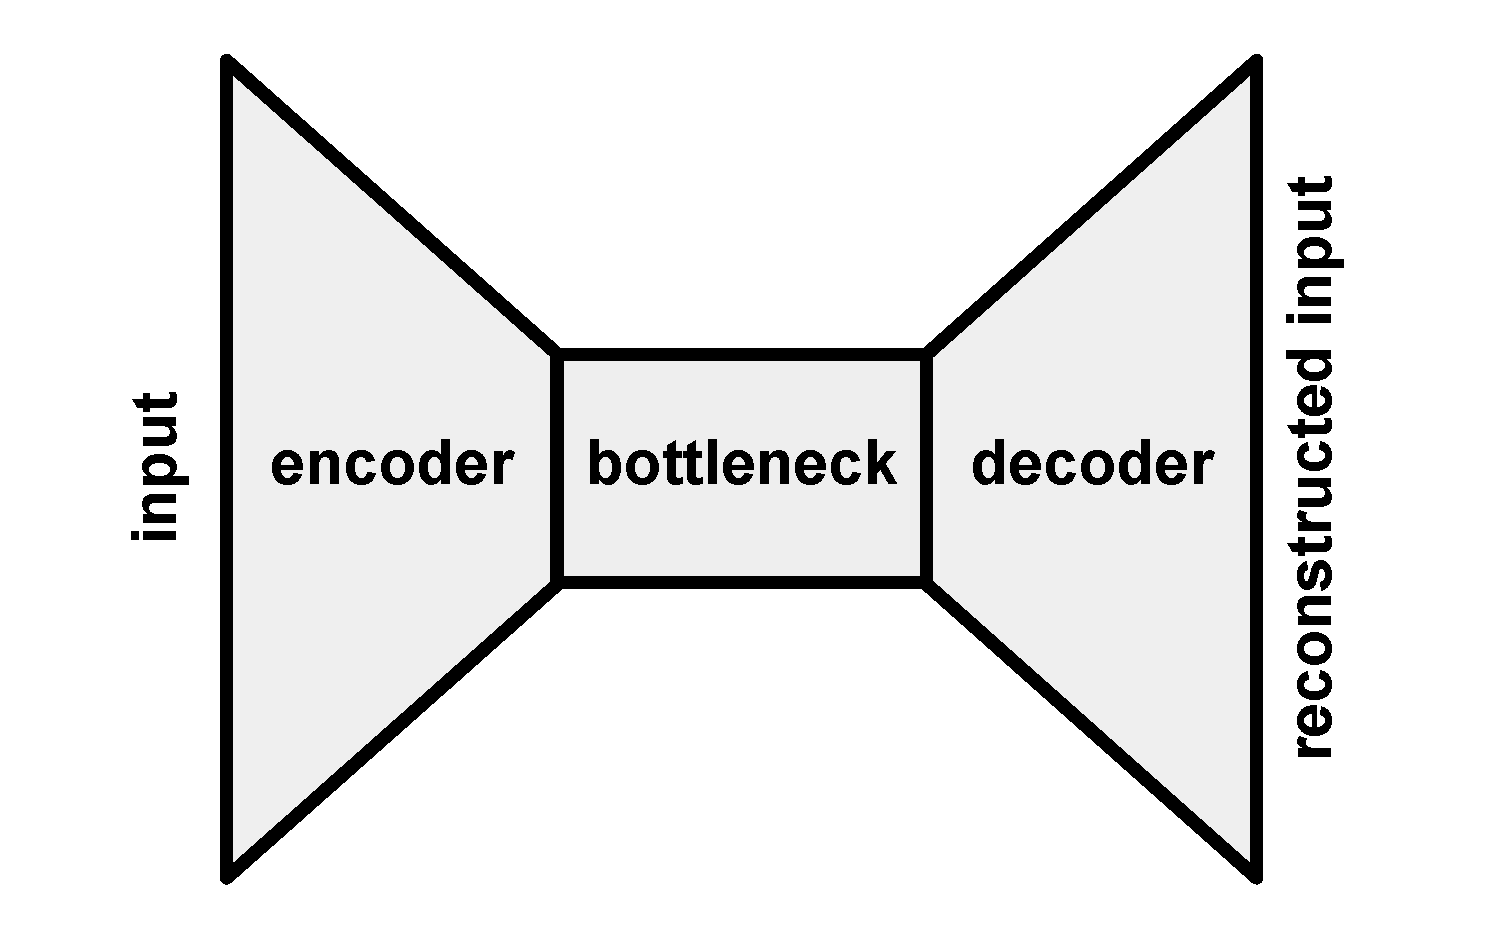
\includegraphics[width=0.5\linewidth]{img/bottleneck}
  \caption{Schematic of a bottlenecked autoencoder.}
  \label{fig:bottleneck}
\end{figure}


The first technique uses a bottlenecked autoencoder.
Figure \ref{fig:bottleneck} provides a schematic impression of such an autoencoder.
This autoencoder has a small layer in the middle that information must pass through to reach the output.
Thus, the autoencoder is forced to learn a compact representation for the input it is trained with that can pass through the bottleneck.
The part of the autoencoder that precedes the bottleneck is called the encoder and the part that follows is called the decoder.
This autoencoder will be trained to encode phenotypes taken from fitness peaks throughout an evolutionary search space.
The idea of this approach is that, because the bottleneck provides a compact representation of those high-fitness phenotypes, using the decoder as a genotype-phenotype mapping will readily allow mutation to move the phenotype between otherwise distant fitness peaks.

\begin{figure}
  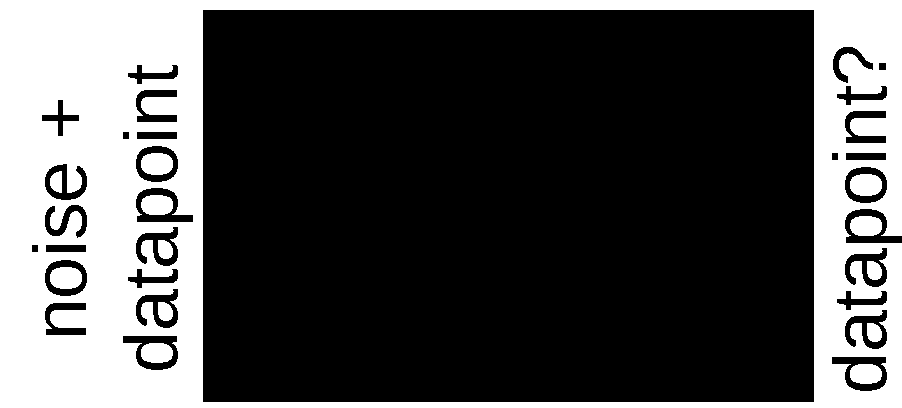
\includegraphics[width=\linewidth]{img/denoiser}
  \caption{
    Schematic of a denoising autoencoder.
  }\label{fig:denoiser}
\end{figure}


The second technique uses a denoising autoencoder.
Figure \ref{fig:denoiser} provides a schematic depiction of such an autoencoder.
These autoencoders have not bottleneck.
Instead, they are trained to reconstruct noisy input into its original unadulterated form.
This autoencoder will be trained to reconstruct phenotypes taken from fitness peaks throughout an evolutionary search space.
For this approach, the entire denoising autoencoder would be used as the genotype-phenotype mapping.
The idea of this design is that mutations that would otherwise be deleterious will effectively be interpreted as noise and prevented from being expressed by the genotype-phenotype mapping.
Effectively, this mapping should flatten out the valleys between local fitness peaks to allow evolution to more readily drift between those local fitness peaks.


\subsection{Learning an Evolvable Genotype-Phenotype Mapping}


% \section{Toy Problem Description} \label{sec:problem-description}

A simple problem will be used as proof of concept.
This problem, the $n$-legged table problem, models a table design scenario where selection is made for the height of the table and it is highly disadvantageous to have different-length legs.
In this case, short tables will be selected for over tall tables.

In the phenotype space, solutions are a $n$-length bitstring.
The $i$th bit of the bitstring represents whether the the $i$th leg of the table is in the long or short configuration.

In this problem, phenotypic novelty can be measured by the hamming distance between two phenotypes.

The cost function will be defined as,
\begin{align*}
C(l_1, l_2, \ldots, l_n)
&=
\alpha \sum_{i = 1}^{n} l_i
+
\sum_{i=1}^n \Big[l_i - \Big(\frac{1}{n} \sum_{j=1}^n l_j\Big)\Big]^2
\end{align*}
where $\alpha$ is a parameter that controls how strongly favored short tables are over tall tables.
Fitness will be inversely proportional to cost.
As selection will be performed by tournament, only relative --- not absolute fitness --- is of concern.

Suppose $n=4$ and $\alpha = \frac{1}{10}$.
Then, we can tabulate the cost for having different leg combinations
\begin{center}
\begin{tabular}{ c c c }
 $C$ & short legs & long legs \\
 0.20 & 0 & 4 \\
 0.40 & 1 & 3 \\
 0.43 & 2 & 2 \\
 0.30 & 3 & 1 \\
 0.00 & 4 & 0
\end{tabular}
\end{center}
Thus, we can see that the fitness landscape is deceptive.
Although the global minimum cost occurs with four short legs, initially converting long legs to short legs results in an increased cost.
A similar calculation shows that increasing alpha decreases the deceptiveness of the search space.

%
% \section{Approach} \label{sec:approach}

The two proposed genotype-phenotype map learning techniques are based on artificial neural network autoencoders.
These are networks that are trained to regurgitate as output the input that they were provided.
Such networks are used to discover efficient lower-dimensional codings for datasets and, more recently, as method for generative modeling \cite{liou2014autoencoder, kingma2013auto}.

\begin{figure}
  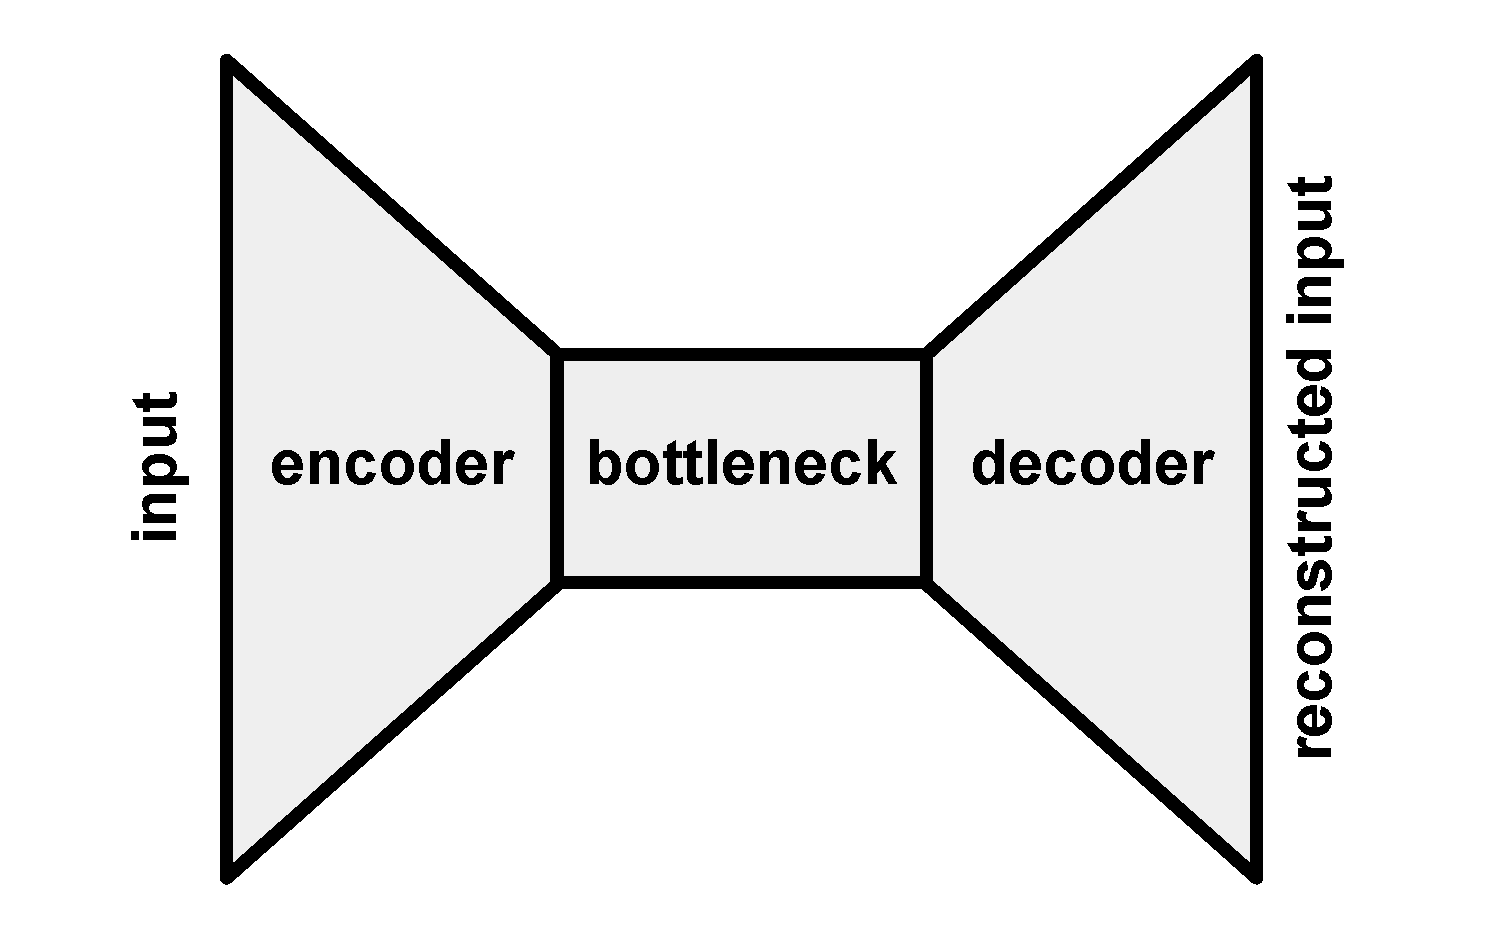
\includegraphics[width=0.5\linewidth]{img/bottleneck}
  \caption{Schematic of a bottlenecked autoencoder.}
  \label{fig:bottleneck}
\end{figure}


The first technique uses a bottlenecked autoencoder.
Figure \ref{fig:bottleneck} provides a schematic impression of such an autoencoder.
This autoencoder has a small layer in the middle that information must pass through to reach the output.
Thus, the autoencoder is forced to learn a compact representation for the input it is trained with that can pass through the bottleneck.
The part of the autoencoder that precedes the bottleneck is called the encoder and the part that follows is called the decoder.
This autoencoder will be trained to encode phenotypes taken from fitness peaks throughout an evolutionary search space.
The idea of this approach is that, because the bottleneck provides a compact representation of those high-fitness phenotypes, using the decoder as a genotype-phenotype mapping will readily allow mutation to move the phenotype between otherwise distant fitness peaks.

\begin{figure}
  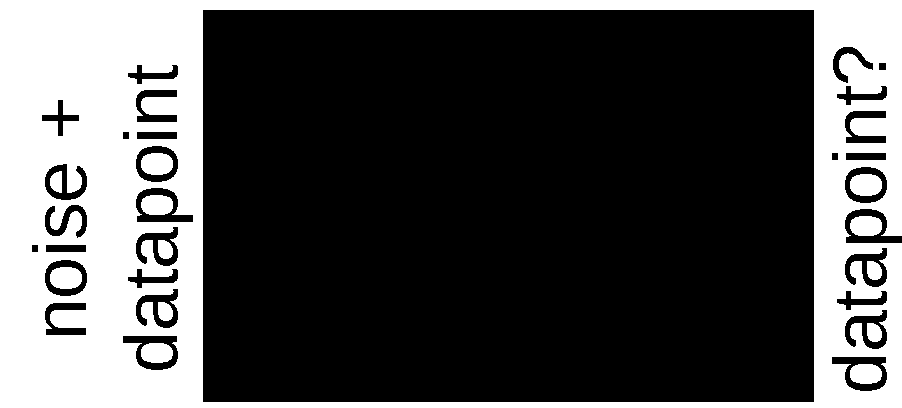
\includegraphics[width=\linewidth]{img/denoiser}
  \caption{
    Schematic of a denoising autoencoder.
  }\label{fig:denoiser}
\end{figure}


The second technique uses a denoising autoencoder.
Figure \ref{fig:denoiser} provides a schematic depiction of such an autoencoder.
These autoencoders have not bottleneck.
Instead, they are trained to reconstruct noisy input into its original unadulterated form.
This autoencoder will be trained to reconstruct phenotypes taken from fitness peaks throughout an evolutionary search space.
For this approach, the entire denoising autoencoder would be used as the genotype-phenotype mapping.
The idea of this design is that mutations that would otherwise be deleterious will effectively be interpreted as noise and prevented from being expressed by the genotype-phenotype mapping.
Effectively, this mapping should flatten out the valleys between local fitness peaks to allow evolution to more readily drift between those local fitness peaks.

%
% \section{Methods} \label{sec:methods}

In this Section, we begin with a high-level overview of each variant of the Automap approach.
Then, we discuss two problem domains used to demonstrate these methods --- the $n$-legged table problem and the Scrabble string problem.
We cover the specific implementation of Automap employed in each of those domains.
Finally, we review a visualization technique called the evolvability signature, which we will later use to examine the evolvability properties of genotype-phenotype maps in both problem domains  \cite{tarapore2015evolvability}.

\subsection{Learning an Evolvable Genotype-Phenotype Mapping}

The pair of proposed techniques to automatically learn evolvable genotype-phenotype mappings are based on autoencoders trained to encode phenotypes taken from local fitness peaks spread throughout an evolutionary search space.
(These phenotypes are gathered by evolving a large number of replicate direct-encoded populations and retaining champion individuals from each population).

\begin{figure}
  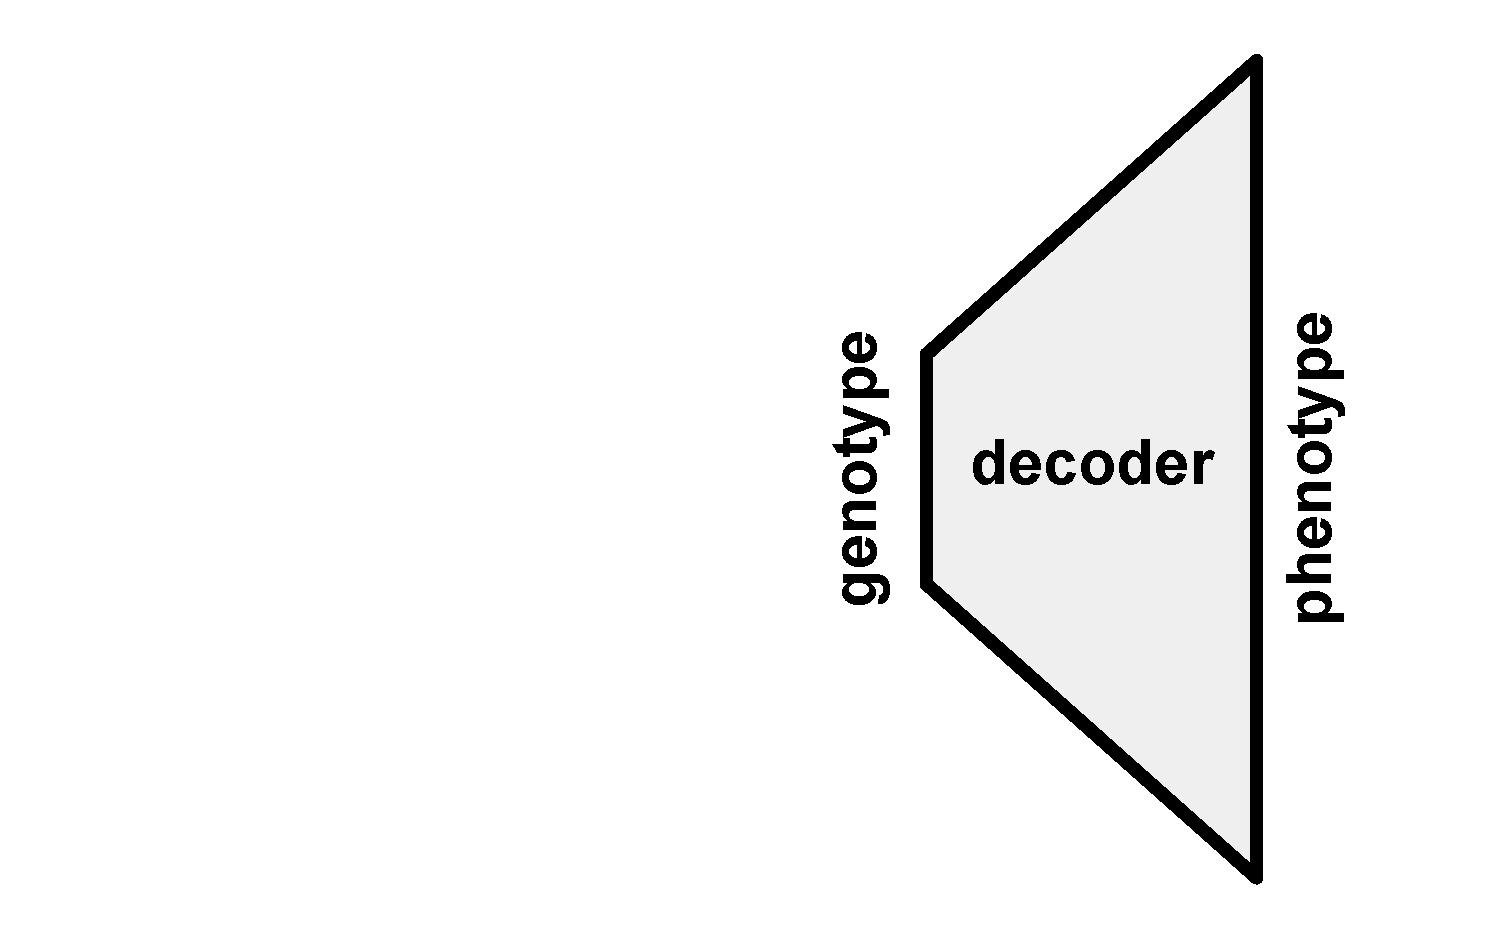
\includegraphics[width=\linewidth]{img/bottleneck_map}
  \caption{Schematic of a genotype-phenotype map constructed with a bottlenecked autoencoder.}
  \label{fig:bottleneck_map}
\end{figure}


The first approach, the bottleneck map, uses just the decoder portion of the bottleneck autoencoder.
The decoder serves as the genotype-phenotype map so the genotype is now in the bottleneck vector space while the phenotype remains in the same vector space as before.
The idea of this approach is that, because the bottleneck provides a compact representation of those high-fitness phenotypes, using the decoder as a genotype-phenotype mapping will readily allow mutation to move the phenotype between otherwise distant fitness peaks.
This approach is illustrated in Figure \ref{fig:bottleneck_map}.

\begin{figure}
  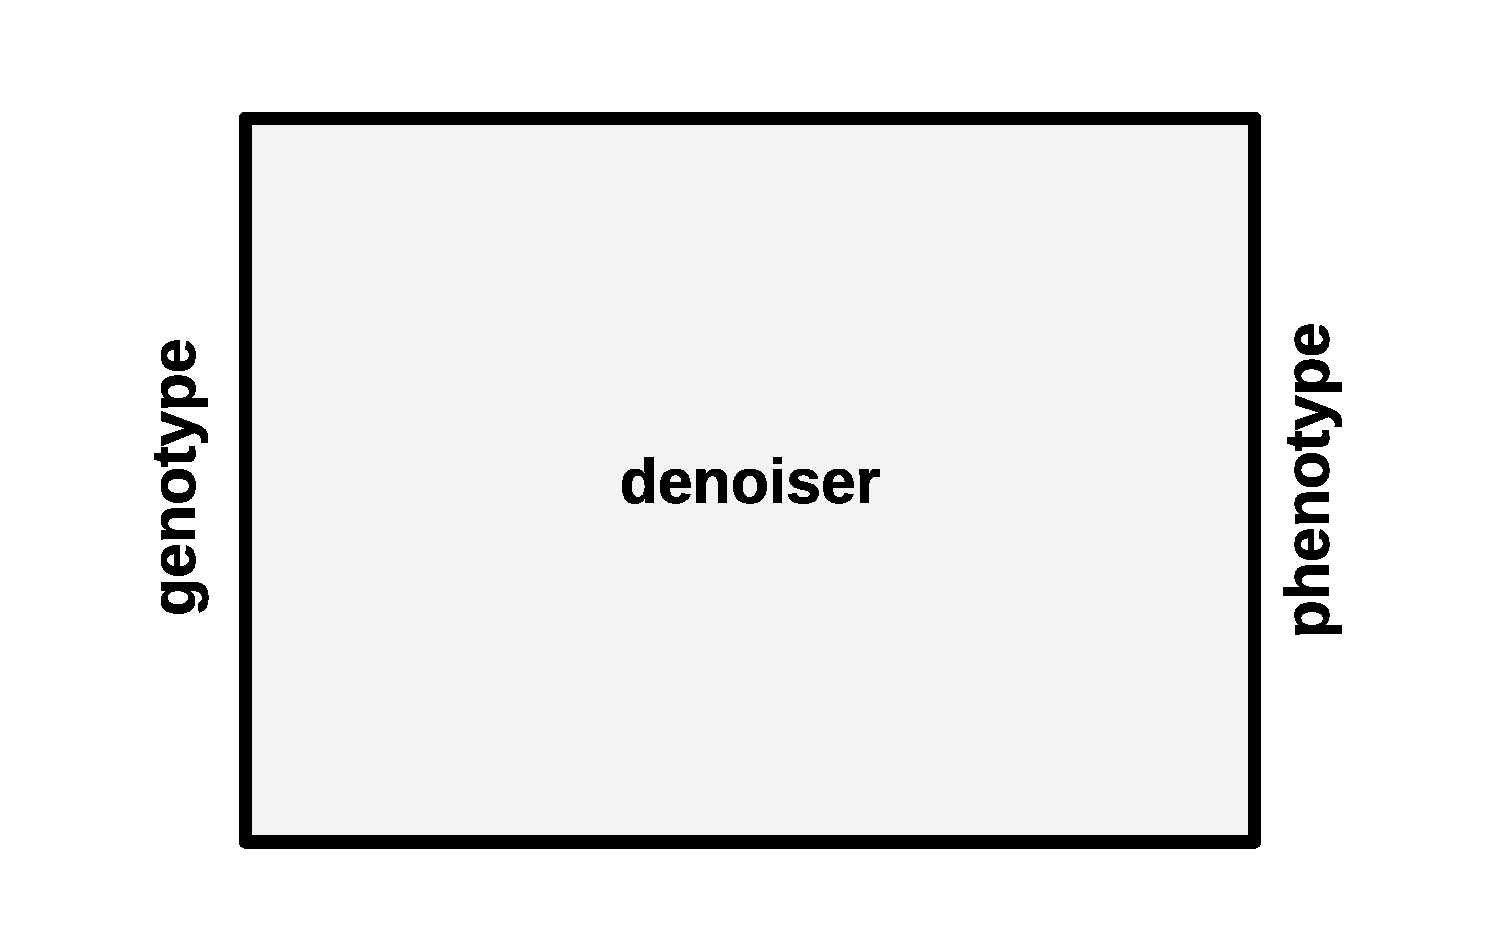
\includegraphics[width=\linewidth]{img/denoiser_map}
  \caption{
    Schematic of a genotype-phenotype map constructed with a denoising autoencoder.
  }\label{fig:denoiser_map}
\end{figure}


The second approach, the denoiser map, employs the entire denoising autoencoder would be used as the genotype-phenotype mapping.
Note that the genotype and phenotype remain in the same, equivalent vector spaces.
The idea of this design is that mutations that would otherwise be deleterious will be interpreted as noise and prevented from being expressed by the genotype-phenotype mapping.
Effectively, this mapping should flatten out the valleys between local fitness peaks to allow evolution to more readily drift between those local fitness peaks.
This approach is illustrated in Figure \ref{fig:denoiser_map}.

\subsection{$n$-legged Table Problem}

This simple problem is used to present a proof-of-concept for the proposed AutoMap techniques.
The $n$-legged table problem models a table design scenario.
In this problem, the phenotype of a table is nothing more than a collection of continuous-valued individual leg lengths.
All other details of table design are neglected.
Stability is considered a highly-advantageous trait for a table.
The stability of a table is assumed to result solely from uniformity of table leg lengths.
Clearly, as $n$ grows beyond eight or so this toy problem begins to lose a meaningful connection to real world tables.
(When was the last time you saw a fifty-legged table?)
However, mathematically (and intuitively) the $n$-legged table problem scales easily.
We arbitrarily use $n=100$ for all experiments in this domain.

This toy problem was chosen because it creates an easy-to-understand rugged fitness landscape.
Because unstable tables are disadvantageous, mutations to level tables tend to be deleterious.
Thus, evolving between different table heights --- i.e. escaping local maxima --- is a tricky challenge.

For evolvability signature experiments, ``level-ness'' was the sole criterion for fitness.
For a phenotype $\vec{x}$, the fitness score was computed as
\begin{align*}
-\sigma(\vec{x})
\end{align*}
where $\sigma$ represents calculation of standard deviation.
Note that in all experiments performed, selection was performed to maximize (not minimize) fitness score.
Under this criterion, each level table of a particular height is a local fitness peak because any single-site mutation increases the leg height variance.
This fitness criteria was chosen for evolvability signature experiments because of its ruggedness.

For response to selection experiments, the ``level-ness'' and absolute height of a table were both factored into the fitness score.
For a phenotype $\vec{x}$, the fitness score was computed as
\begin{align*}
-\sigma(\vec{x}) - |\mu(\vec{x})/10|
\end{align*}
where $\sigma$ represents calculation of standard deviation and $\mu$ represents calculation of mean.
Under this criterion, a selection pressure for short tables is applied.
The global fitness score peak is the table with all legs length 0.
However, the phenotypic fitness landscape remains rugged with local peaks occurring as before at level tables.
Thus, the ability of genotype-phenotype map to facilitate evolution will be reflected by the ability of a population to escape local fitness peaks and progress towards the global fitness peak.

\subsection{Scrabble String Problem}

The Scrabble string problem provides a more challenging testbed for the AutoMap approach.
In this problem domain, phenotypes are 100-character strings consisting of the letters ``a'' through ``z'' and the `` '' (space) character.
Fitness is determined as the count of letter characters contained in valid Scrabble words within the 100-character string.
First and foremost, this problem was chosen because phenotypes --- and potential indirect genotype-phenotype maps --- were thought likely to be easily human-understandable.
This problem also serves as a rough stand-in for linear genetic programming; both revolve around evolving sequences of symbols.
Finally, working in this problem domain allowed us to leverage existing deep learning work with character-level representations of English language \cite{weiss2016spellling}.
Like the $n$-legged table problem, the Scrabble string problem presents a rugged fitness landscape.
Many changes to components to the phenotype that are part of a valid scrabble word will invalidate the word, sharply reducing the string's count of letter characters contained in valid Scrabble words.
Thus, many mutations will have severely deleterious consequences.

\subsection{Implementation}

The evolutionary computing components of this project were implemented using the Distributed Evolutionary Algorithms for Python package, which allows for rapid prototyping and extreme flexibility \cite{fortin2012deap}.
The artificial neural network autoencoder components of this project were implemented using PyTorch, a Python-based deep learning framework \cite{paszke2017pytorch}.

\subsubsection{$n$-legged Table Problem}

For the $n$-legged table problem, the denoising autoencoder consisted of a 100-to-100 fully-connected linear layer without bias.
The network was trained for 2500 epochs by stochastic gradient descent with learning rate: $1^{-4}$, momentum $0.9$, and batch size $2048$.
Model parameters were initialized uniformly between $0.005$ and $0.015$.
During training, parameters were clamped in the range $(0,1)$.
During the training process, Gaussian noise with $\mu = 0, \sigma = 0.025$ was introduced to the input presented to the autoencoder.
Loss was defined as mean square error of the difference between the original phenotype the reconstructed phenotype.

For the $n$-legged table problem, the bottleneck autoencoder consisted of a 100-to-1 fully-connected linear layer with bias (encoder) and a 1-to-100 fully-connected linear layer with bias (decoder).
Thus, the bottleneck consisted of 1 float value.
The network was trained for 200 epochs by stochastic gradient descent with learning rate $1^{-3}$, momentum $0.7$, and batch size $16$.
Loss was defined as mean square error of the difference between the presented phenotype and the reconstructed phenotype.

For the $n$-legged table problem, training data for both encoders was generated from 250 populations of 300 individuals evolved with direct genotype-phenotype map.
Initial leg lengths of each separate population were taken from a Gaussian random walk seeded uniformly between $0$ and $1000$ with $\mu = 0, \sigma = 1.0$ where each set of 100 consecutive values was taken as the initial leg lengths of a particular individual.
This step was performed to ensure that the 250 populations were well-spread throughout the phenotype space.
The 250 populations were evolved separately for 50 generations using the operators and settings described for the direct encoding for the evolvability signature experiments.
The 7500 phenotypes --- vectors of 100 float values --- present in the populations after 50 generations of evolution were taken as training data.
Leg length values were normalized to the range $(0,1)$ for the training process.
Both encoders were easily trained on a PC (no GPU).

For all $n$-legged table experiments, tournament selection with $k = 5$ was used.
With probability $0.5$, offspring engaged in two-point crossover with one other individual.
(Note, though, that when the bottleneck genotype-phenotype is was employed the genotype is a member of $\mathcal{R}$ so crossover has no effect.)
Mutation was performed by site-wise Gaussian perturbation of the genome.
For evolvability signature experiments, mutation of genome elements was $\mu=0, \sigma=0.1$ with a per-individual probability of $0.2$ and a subsequent per-site probability of $0.01$.
For response to selection experiments, mutation of genome elements was $\mu=0, \sigma=0.1$ with a per-individual probability of $0.2$ and a per-site probability of $0.2$.
(For all experiments with the bottleneck map, a per-site probability of $1$ $\sigma=0.1$ was employed.)
These particular operators were used due to their easy accessibility in DEAP.
As these experiments were demonstrative instead of applied, the primary criteria
for operators and parameters needed to meet was simply not being obscure enough to distract from the new genotype-phenotype mapping techniques being demonstrated.
It would be beneficial to repeat these experiments with other operator and parameter choices popular in the literature and in applied use to investigate the generalizability of those new techniques.

\subsubsection{Scrabble String Problem}

For the Scrabble string problem, the denoising autoencoder consisted of: a 9,000-channel 1-dimensional convolution layer with kernel size 3, a ReLU layer, a 100-channel 1-dimensional convolution layer with kernel size 5, a ReLU layer, a 1500-to-1500 fully connected linear layer with bias, a Tanh layer, and a 1500-27 fully connected linear layer with bias.
Initial model weights were drawn from the standard normal distribution.
To generate training data, 20,000 direct-encoded populations of 100-character strings were evolved for 40,000 generations.
During training, input to the autoencoder were 15-character substrings of champion phenotypes with each character encoded as a one-hot vector.
With probability 0.25, the middle character of the presented substring was redrawn.
Over the course of two days, the network was trained for 4 epochs on a GPU-accelerated machine with the Adam optimizer and batch size 256.
Loss was defined as mean square error of the difference between the true identity of the input substring's middle character (before any scrambling) and the predicted identity of that character.
At the conclusion of training, the denoising autoencoder predicted the correct identity of the substring's middle character at a rate of approximately 85\% on testing data.
Example input/output of the denoising autoencoder during training is shown in Figure TODO.
For the Scrabble string problem, each site of the 100-character genotype was fed through the denoiser, yielding a new 100-character string that consisted of the denoiser's prediction at each site.
Figure TODO illustrates this process.
The denoiser genotype-phenotype mapping was achieved by performing four of these denoising passes on the genotype.

For all Scrabble string experiments, tournament selection with $k = 3$ was used.
No crossover was performed.
(Note, though, that when the bottleneck genotype-phenotype is was employed the genotype is a member of $\mathcal{R}$ so crossover has no effect.)
Mutation was performed by site-wise Gaussian perturbation of the genome.
Mutations scrambled a single, randomly-chosen character in the genotype.
We applied a per-individual mutation rate of 0.2 and a per-site mutation rate of 0.1 while evolving training data for the denoiser.
For all other experiments, we used a per-individual mutation rate of 0.33 and a per-site mutation rate of 0.01.
These particular operator and parameter choices were made mainly by happenstance --- as before, it would be beneficial to repeat these experiments with other operator and parameter choices.

\subsection{Evolvability Signature}
Tarapore et al. introduced an evolvability measure that enables simultaneous inspection of both major aspects of evolvability --- viability and novelty of phenotypic outcomes under mutation \cite{tarapore2015evolvability}.
They forgo use of a scalar metric to describe evolvability, instead reporting evolvability using what they term a ``signature.''
Essentially, the signature is a two-dimensional heatmap presenting the changes in phenotypic form and fitness observed in individual offspring from a single parent.
Normalized mutual information between the phenotypic states of parent and offspring is used to quantify the amount of change in phenotypic form observed in an offspring.
Proportion decrease in fitness is used to quantify the fitness difference between parent and offspring.
For a highly evolvable individual, we would expect to see offspring occurring with significant frequency in the corner of the heatmap indicating significant change in phenotypic form with slight or no loss of fitness.
The evolvability signature provides a nuanced snapshot of evolvability, allowing for interaction between the two primary components of evolvability to be visualized.
Such information can be highly diagnostic, for example alerting researchers to phenomena that might appear falsely promising using other metrics, such as genetic changes that alter phenotypic form significantly but at great cost to fitness or genetic changes that are beneficial to fitness but fail to uncover novel phenotypic form.
Figure \ref{fig:reading_evolvability_signature} illustrates how an evolvability signature is laid out.

\begin{figure}
  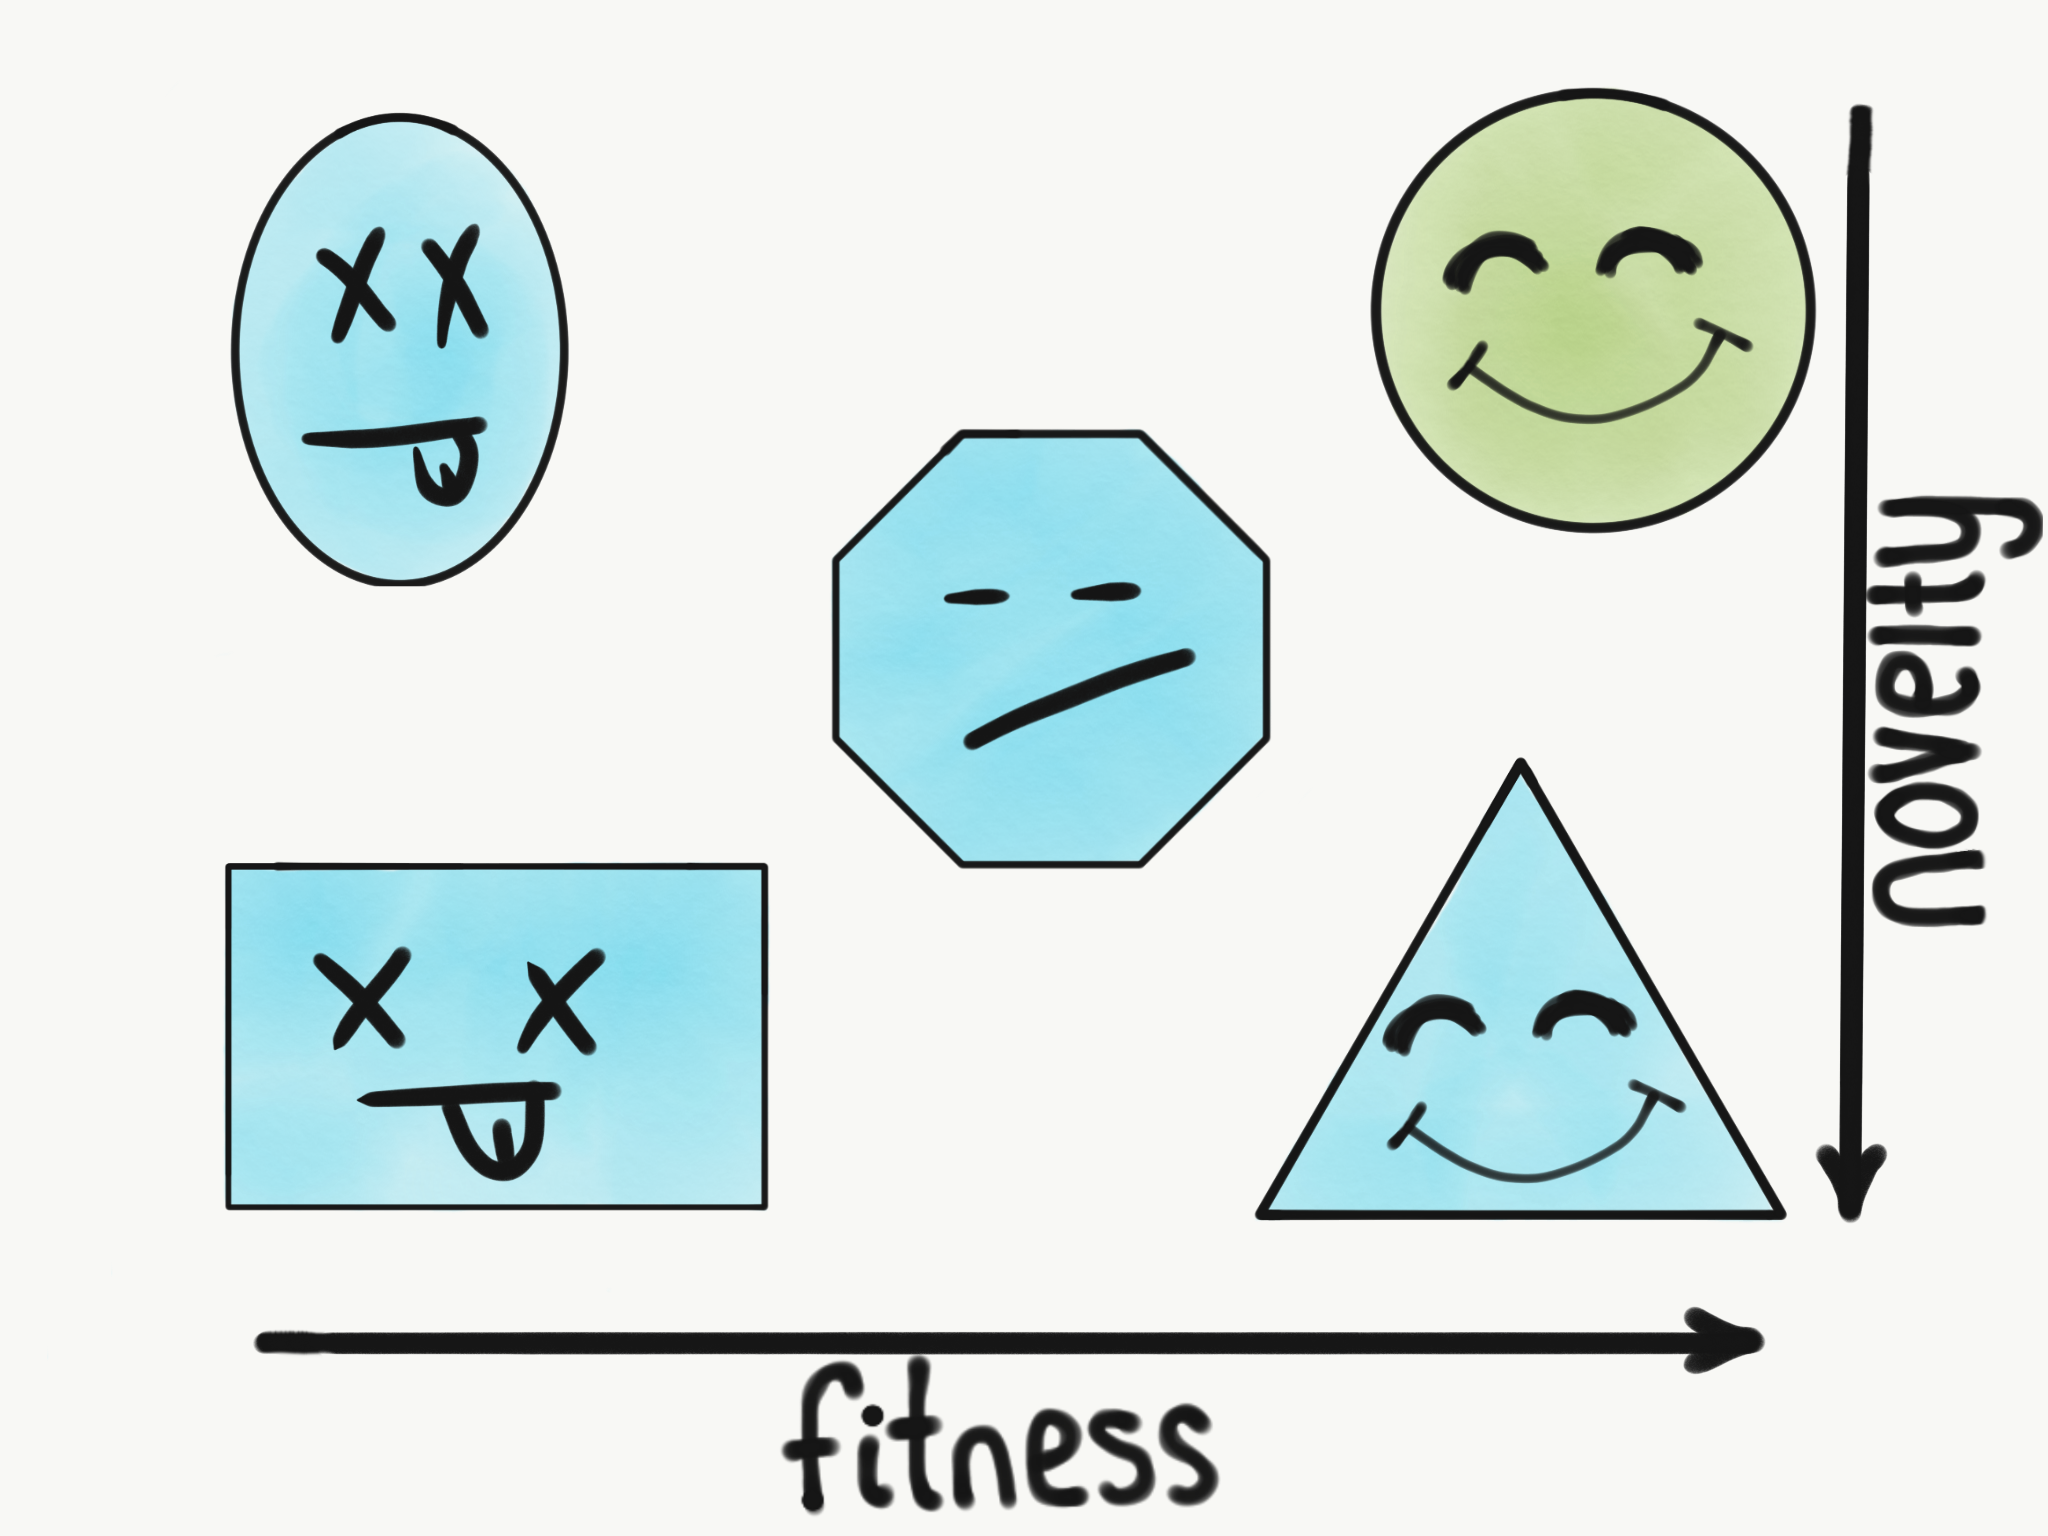
\includegraphics[width=0.8\linewidth]{img/reading_evolvability_signature}
  \caption{
    Cartoon illustration describing the layout of an evolvability signature diagram \cite{tarapore2015evolvability}.
    The parent phenotype is located in the upper right.
    Novelty increases top to bottom and fitness decreases right to left.
  }\label{fig:reading_evolvability_signature}
\end{figure}


%
% \section{Results and Discussion} \label{sec:results}

\subsection{$n$-legged Table Problem}

\begin{figure*}
  \begin{subfigure}[b]{0.33\linewidth}
    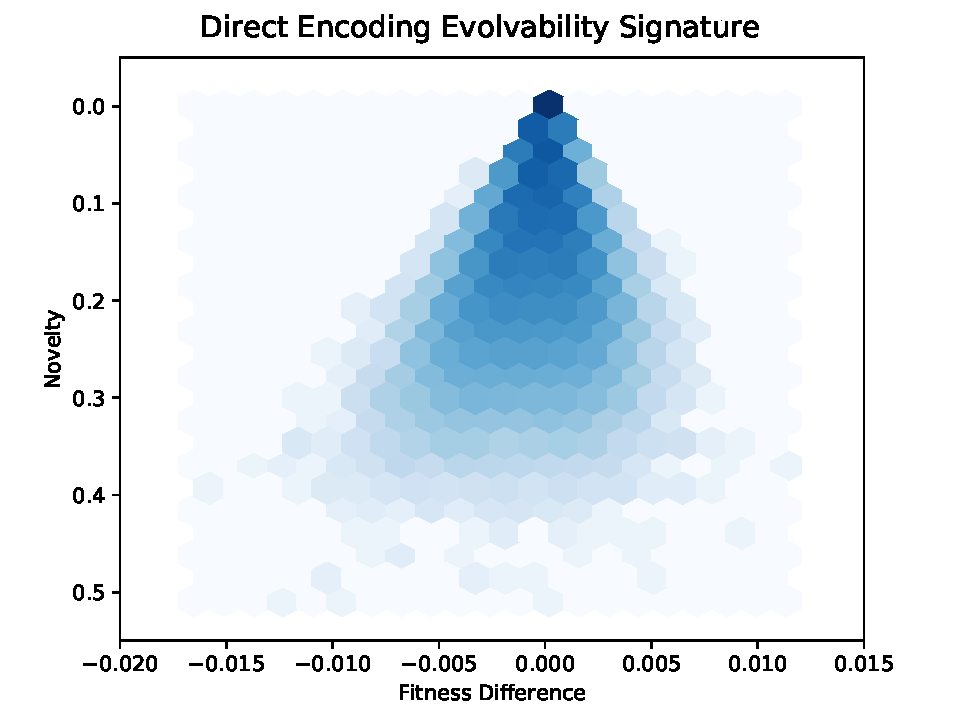
\includegraphics[width=\linewidth]{img/direct_es_unscaled}
    \subcaption{
      direct map
    }\label{fig:table_direct_es}
  \end{subfigure}
  \begin{subfigure}[b]{0.33\linewidth}
    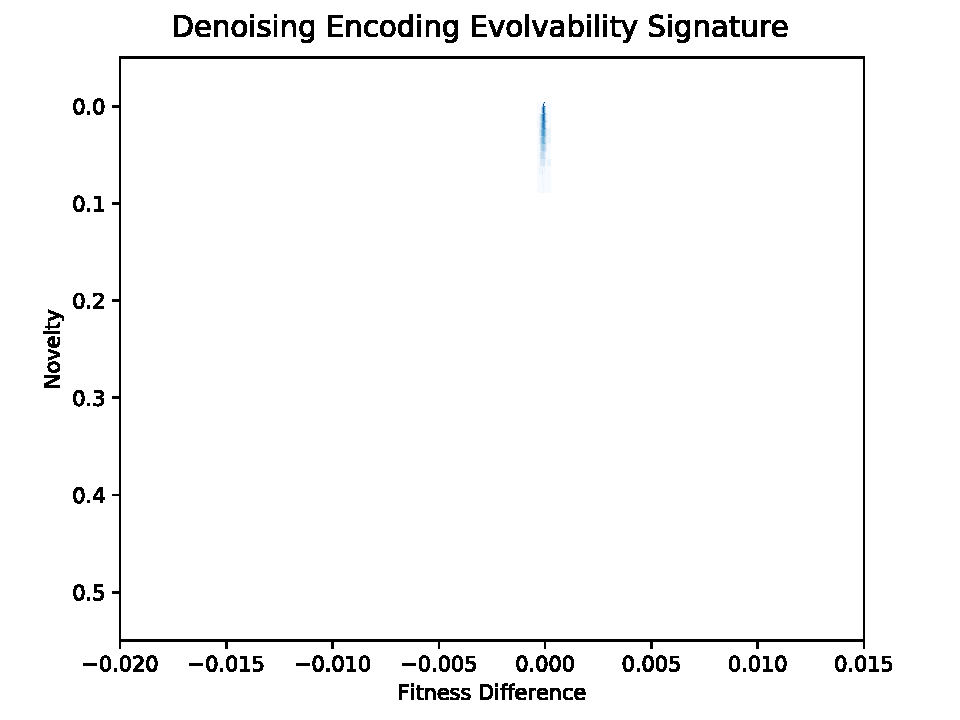
\includegraphics[width=\linewidth]{img/noise_es_unscaled}
    \subcaption{
      denoising map
    }\label{fig:table_noise_es}
  \end{subfigure}
  \begin{subfigure}[b]{0.33\linewidth}
    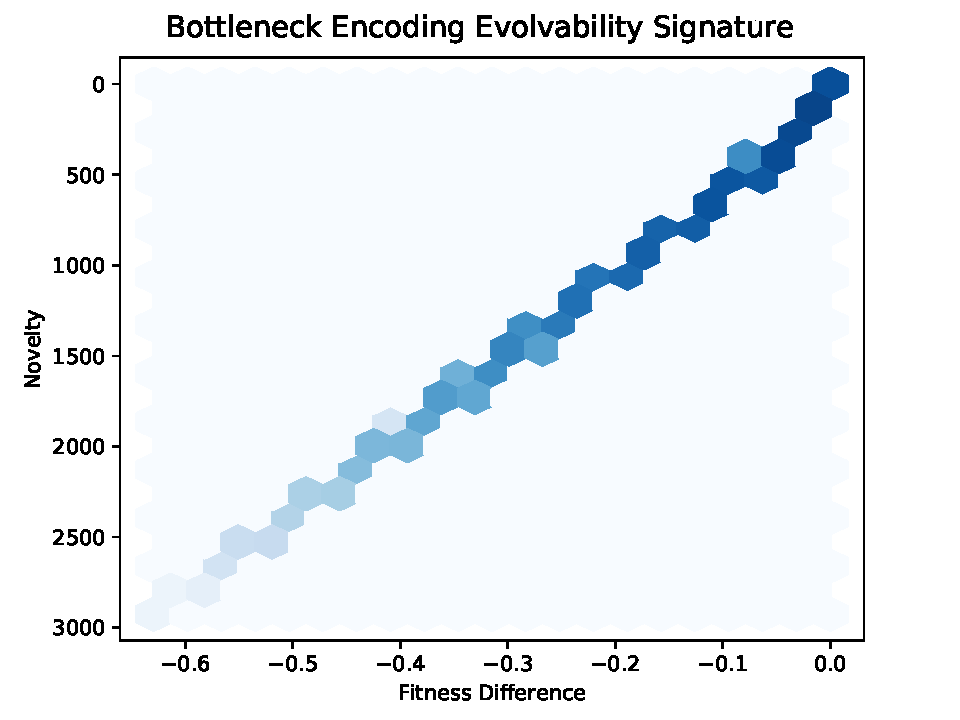
\includegraphics[width=\linewidth]{img/bottleneck_es_unscaled}
    \subcaption{
      bottleneck map
    }\label{fig:table_bottleneck_es}
  \end{subfigure}
  \caption{
    Evolvability signatures for three genotype-phenotype maps in the $n$-legged table problem domain.
    Note that subfigure \ref{fig:table_bottleneck_es} is presented with different axis scaling than subfigures \ref{fig:table_direct_es} and \ref{fig:table_noise_es}.
  }\label{fig:all_es}
\end{figure*}


We used evolvability signature analysis to characterize the evolvability of the $n$-legged table direct, bottleneck, and denoiser encodings (Figure \ref{fig:all_es}).
The bottleneck mapping clearly generates more novelty per mutational step than either of the other mappings.
Fitness does decline in tandem with novelty, but the absolute fitness scores of all mutant offspring under the bottleneck mapping are greater than the absolute fitness of the direct-evolved champions.
Relatedly, although beneficial mutational outcomes are observed frequently under the direct encoding this is likely affected by relatively low absolute fitness of $-0.82$ ($s=0.1$) for direct-evolved champions (in comparison, for instance, to absolute fitness of $-0.025$, $s=0.004$ for denoiser-evolved champions).
Finally, more novelty is produced by mutation under the direct encoding compared to the denoising encoding.
The denoiser's action filtering out certain phenotypic variation likely contributes to the reduction of novelty observed under mutation.

\begin{figure}
  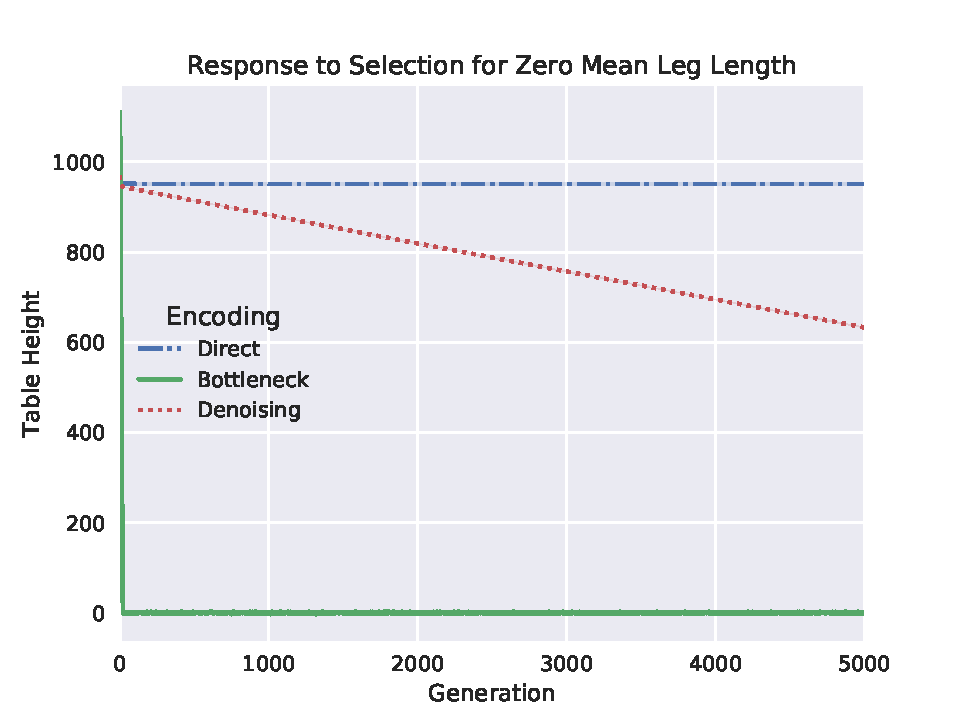
\includegraphics[width=\linewidth]{img/zero_leg_selection}
  \caption{Response to short-table selection pressure under different genotype-phenotype maps.}
  \label{fig:select_response}
\end{figure}


Subsequently, we assessed the ability of the three genotype-phenotype maps to facilitate traversal of the evolutionary search space in response to a selective pressure.
Specifically, a selective pressure for short table height was added.
Table height is calculated as the mean leg length of a table.
For each map, we evolved three replicate populations of 300 individuals for 5,000 generations.
We initialized these populations to have table height of approximately 1,000.
Response to selective pressure for short table height was assessed by tracking mean table height of the populations generation-by-generation.
Figure \ref{fig:select_response} plots mean table height by generation under selection for both zero table height and table stability.
Shaded areas, hugging the table height trajectories so tight as to be difficult to discern, represent bootstrapped 95\% confidence intervals ($n=3$).

Under the direct mapping, a slight decrease in mean table height is observed for a few generations after initialization.
However, no further decrease in mean table height was observed over the course of evolutionary runs.
These runs ended with a mean table height of approximately 950.
Direct-encoded populations were trapped at local fitness peaks and unable to respond to selective pressure for short table height.

Under the bottleneck mapping, a switft decrease in mean table height is observed after initialization.
Well within 100 generations, the populations approached to the global fitness peak of a perfectly level table with height zero.
Populations with the bottleneck mapping were able to quickly respond to selective pressure for short table height.

Finally, under the denoising mapping, a slight drop-off in mean table height is observed after initialization, followed by a steady decrease in table height was observed for the remainder of the evolutionary runs.
These runs ended with a mean table height of approximately 630.
Although not as swiftly as under the bottleneck mapping, under the denoising mapping populations were still able to respond to selective pressure for short table height.

Cursory inspection of input/output of the decoding component of the bottleneck autoencoder revealed that it had learned to echo the single bottlenecked float in order to uniformly populate the vector of 100 phenotypic leg lengths.
Thus, the bottleneck genetic representation essentially described the table height; table leg lengths were set using this height value via the genotype-phenotype map.
Evolvability signature analysis suggests that this encoding allows the generation of greater novelty with less deleterious consequence.
Indeed, as in Figure \ref{fig:select_response}, table populations using this encoding are able to rapidly evolve to a global fitness peak.
Similar inspection of the denoising autoencoder revealed that that neural network had essentially learned to calculate each phenotypic leg length output as the average of its inputs.
Thus, the denoising encoding took genetic input for what --- under the direct encoding --- would otherwise be an unstable table and output a stable table nearby in phenotype space.
Evolvability signature analysis shows that although this encoding does not enhance the novelty of phenotypic outcomes under mutation relative to the direct encoding, it does curb the deleterious effects of mutation.
Thus, as in Figure \ref{fig:select_response}, table populations using this encoding are able to make slow and steady progress towards a global fitness peak.

\subsection{Scrabble String Problem}

\begin{figure}
  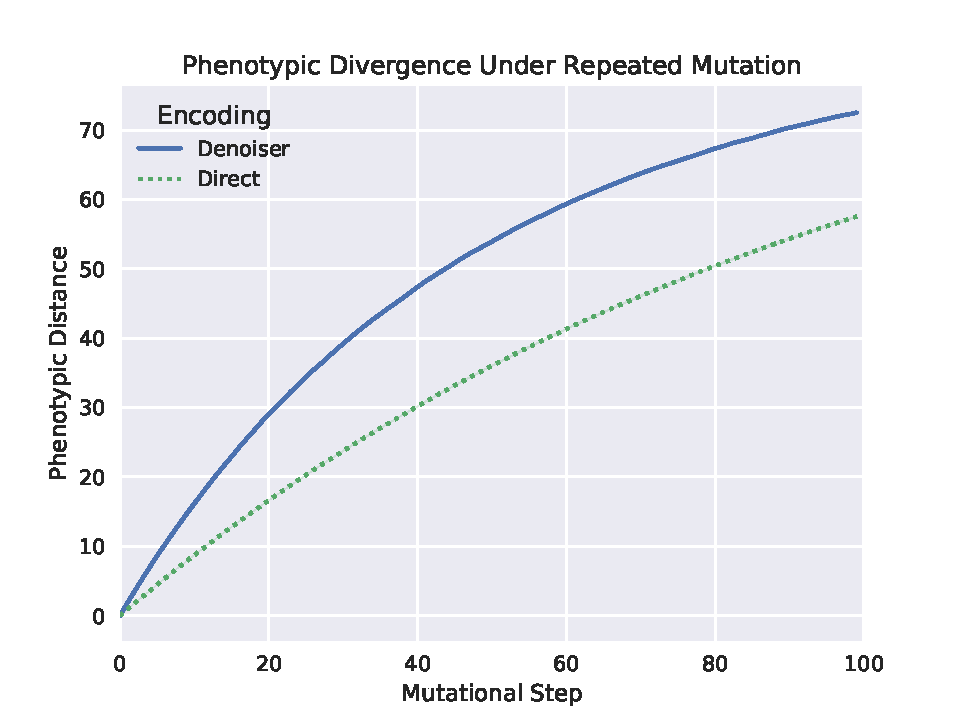
\includegraphics[width=\linewidth]{img/scrabble_dist_vs_step}
  \caption{TODO}
  \label{fig:scrabble_dist_vs_step}
\end{figure}

\begin{figure}
  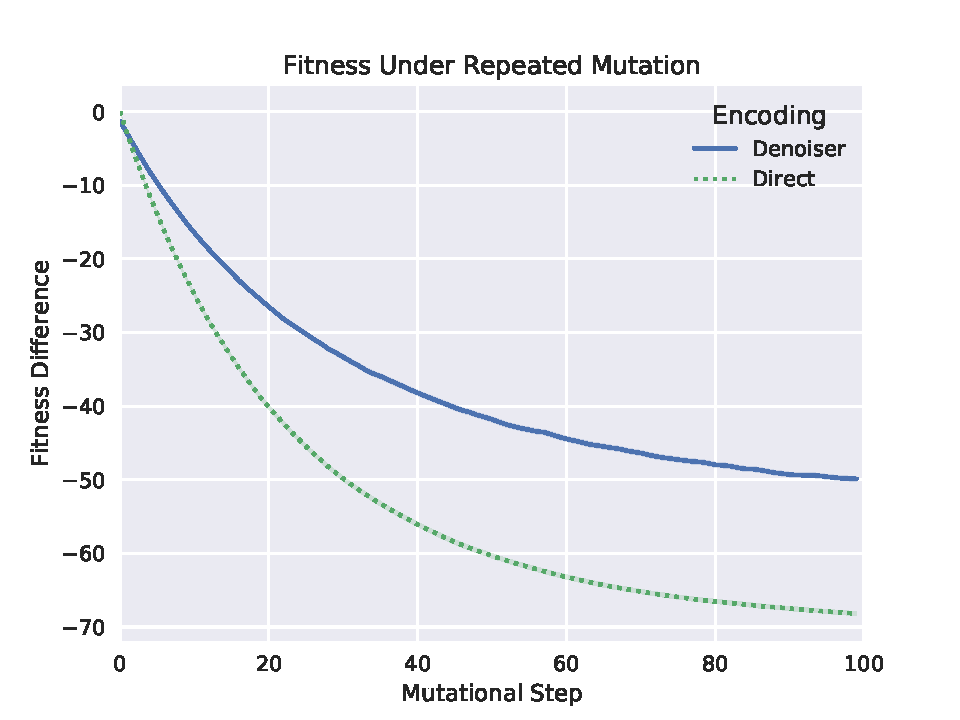
\includegraphics[width=\linewidth]{img/scrabble_fit_diff_vs_step}
  \caption{Fitness loss by mutational step in the Scrabble string domain.}
  \label{fig:scrabble_fit_diff_vs_step}
\end{figure}

\begin{figure}
  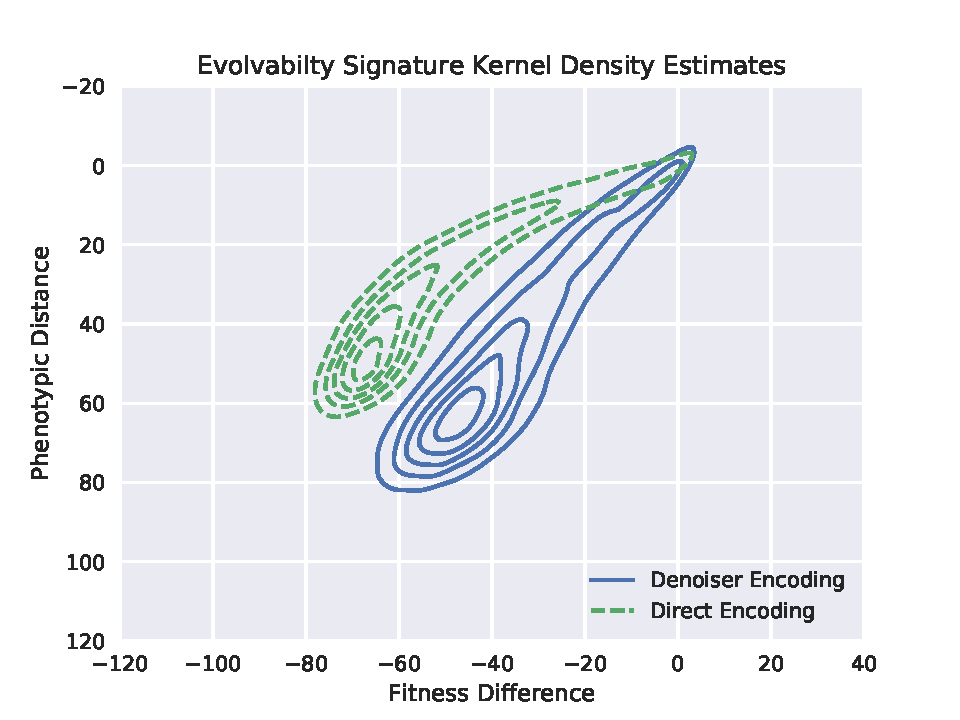
\includegraphics[width=\linewidth]{img/scrabble_es_kde}
  \caption{Gaussian kernel density estimates for evolvability signatures of direct and indirect encodings in Scrabble string domain.}
  \label{fig:scrabble_es_kde}
\end{figure}

\begin{figure}
  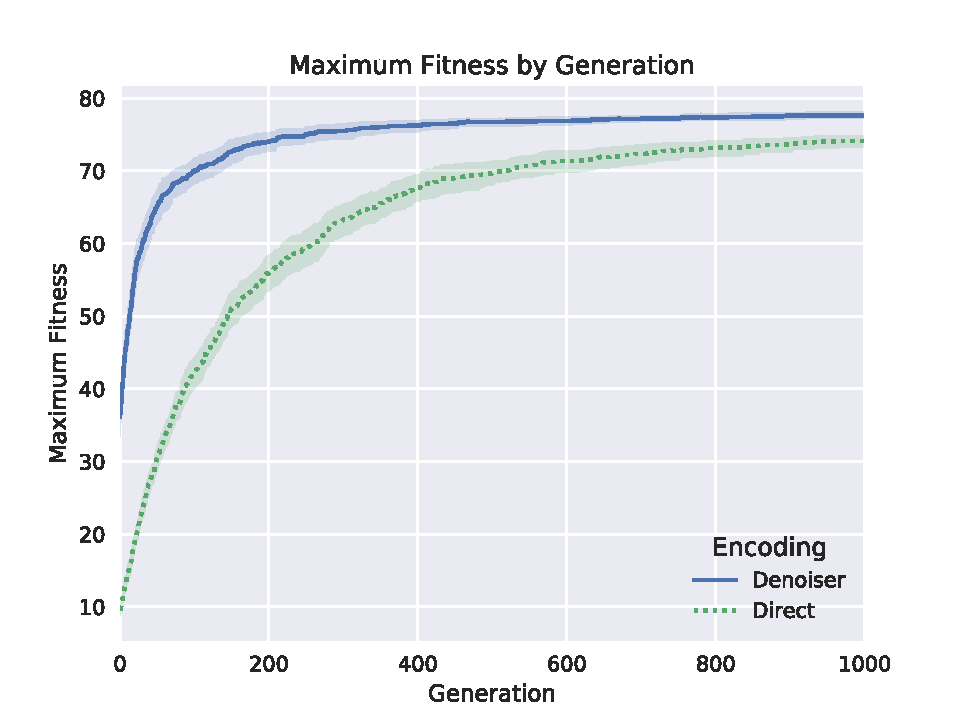
\includegraphics[width=0.8\linewidth]{img/scrabble_fit_vs_gen}
  \caption{
    Maximum individual fitness by generation in populations evolving in the Scrabble string domain.
  }\label{fig:scrabble_fit_vs_gen}
\end{figure}


Evolvability signature analysis was used to characterize the evolvability of the learned denoiser encoding in the scrabble string.
To generate these signatures, 250 champion genotypes were drawn from the direct-encoded populations used to train the denoiser encoding.
100-step mutational walks were then taken from the champion genotype.
The phenotypes generated from those genotypes under both the direct and the denoising encoding were compared.
Figure \ref{fig:scrabble_dist_vs_step} plots novelty (number of non-matching phenotypic characters between the original champion and its mutant offspring) against mutational step ($n=250$).
Novelty increases more rapidly under the denoiser encoding relative to the direct encoding.
Figure \ref{fig:scrabble_fit_diff_vs_step} plots fitness relative to the original champion against mutational step ($n=250$).
Fitness declines more slowly under mutation with the denoiser encoding compared to the direct encoding.
In both of these figures, bootstrapped 95\% confidence are shaded along each curve but are tight enough to be difficult to discern.
Figure \ref{fig:scrabble_es_kde} ties together fitness and novelty information from these random mutational walks in the format of an evolvability signature.
Kernel density estimate contours of evolvability signature densities under both encodings are shown side-by-side.
This comparison shows that the denoiser encoding simultaneously yields more novelty and less fitness decline under mutation.

Subsequently, we tested the capacity of the denoiser encoding to speed up adaptive evolution.
We set up twenty replicate Scrabble string populations to use the the denoiser genotype-phenotype map and twenty Scrabble string populations to use the direct map.
For each population, maximum fitness was recorded over 1,000 generations of evolution.
Figure \ref{fig:scrabble_fit_vs_gen} shows that the populations using the denoiser encoding gain fitness more rapidly than the direct encoding over the first few hundred generations ($n=20$).
(Again, bootstrapped 95\% confidence are shaded along each curve.)
Clearly, the evolvability properties of the denoiser encoding translate to evolutionary dynamics that differ strongly from the direct encoding.

As shown in Figure \ref{fig:scrabble_denoiser}, the denoising autoencoder essentially learns to spell-check a genotype to generate the phenotype.
Generally, though not always, characters contributing to valid words are left undisturbed.
Interestingly, the change that the denoiser makes to correct a spelling error doesn't always reflect the original state of the string.
There are often several possible repairs that will yield valid spelling outcomes.
We hypothesize that this dynamic explains the rapid rate of novelty increase under mutation --- often, instead of correcting the mutated site in the phenotype corrections are applied to one or several \textit{other} sites.
Thus, more than one character in the phenotype may change due to mutation of a single site in the genome.
In particular, based on informal analysis of example sentences fed to it, the denoising autoencoder seems to favor fixing spelling mistakes by strategically replacing a letter character with a space.
This tendency might occur because the denoiser encountered spaces more often than any other single character during training.

%
% \section{Discussion} \label{sec:discussion}

Evolvability signature analysis indicate that, in the $n$-leg table domain, the bottleneck and denoising mapping are both more evolvable than the direct encoding.
The bottleneck mapping allows large mutational steps to be taken through the phenotype space relative to the denoising mapping and the direct mapping.
Both tend to have mutational outcomes that are superior in fitness to those of the direct encoding.
The bottleneck and denoising mappings were observed to free evolution from getting stuck at local fitness peaks, as occurred under the direct mapping, and instead enable progress towards a global fitness peak.
Thus, in the $n$-leg table domain, the proposed genotype-phenotype maps seem to enhance evolvability in both a practical and theoretical sense.

The proposed techniques to generate evolvable genotype-phenotype mappings are in principal generalizable to any context in which many phenotypes at local fitness peaks can be surveyed (i.e. extensive exploratory evolution with a direct encoding isn't computationally prohibitive) and phenotypes can be represented as a continuous-valued, constant-length vector.
Using these techniques may reduce the human labor and expertise required to design evolvable genotype-phenotype mappings for new evolutionary computing domains.
Further, these autoencoder-based approaches might yield more evolvable genotype-phenotype maps than human design for existing evolutionary computing domains.
However, it must be noted that the proposed techniques have only been demonstrated on a toy problem for which it is trivial to manually design an evolvable genotype-phenotype mapping.
Further, it is certainly true that for more complex applications, autoencoder design itself typically requires skilled human input.
Thus, these automatic genotype-phenotype mappings cannot entirely sidestep the need for manual labor.
In fact, in more complex domains, these techniques will introduce a new cost: computation.
Training autoencoders in complex domains, especially the process of developing autoencoder design, will require significant computational resources.

Future work with these autoencoder-based genotype-phenotype maps will focus on demonstrating their utility in more complex domains.
It will be interesting to research how to adapt autoencoder architecture and training to a domain less well-understood than the $n$-leg problem.
For example, questions such as ``What should the size of the bottleneck be for a bottlenecked autoencoder?'' or ``What type of noise should a denoising autoencoder be trained with?'' will need to be addressed.
Ultimately, work should apply these techniques to a domain where human-designed genotype-phenotype mappings have significant shortcomings to attempt to surpass the performance of human-designed maps.

% \end{document}  % This is where a 'short' article might terminate



\appendix
%Appendix A

\begin{acks}
  The authors would like to thank Dr. Yuhua Li for providing the
  MATLAB code of the \textit{BEPS} method.

  The authors would also like to thank the anonymous referees for
  their valuable comments and helpful suggestions. The work is
  supported by the \grantsponsor{GS501100001809}{National Natural
    Science Foundation of
    China}{http://dx.doi.org/10.13039/501100001809} under Grant
  No.:~\grantnum{GS501100001809}{61273304}
  and~\grantnum[http://www.nnsf.cn/youngscientists]{GS501100001809}{Young
    Scientists' Support Program}.

\end{acks}


\bibliographystyle{ACM-Reference-Format}
\bibliography{sample-bibliography}

\end{document}
